\chapter{Rare Event Probabilities}\label{ch:is}
Rare events are events that occur with very low probability.
Such events can be, for example, the die-out of some population or the switching of a multimodal system across some potential barrier.
By their nature, most standard methods focus on regions with high probability.
As an example consider the standard \ac{SSA}:
Trajectories are generated according to the processes density.
Therefore unlikely events are exactly as unlikely to be sampled using the direct method.
Similarly approximations such as moment approximations or mean-field analysis focus on the main probability mass.
Therefore the analysis of such events is particularly difficult.

The arguably most used method for rare event analysis is \acf{IS}.
This variance reduction method is very well-suited to the analysis of such events.
In a nutshell, this method alters the model's dynamics and keeps track of the \emph{likelihood ratio} between this altered and the original model.
This ratio provides an unbiased estimate of the event probability.
The main challenge is to find a good way to alter the model.
One popular approach is found in \acsfont{dwSSA} \parencite{kuwahara2008efficient,daigle2011automated}.
Therein each reaction rate is altered by some constant scalar factor.
These biasing values are identified by using pilot runs of the \ac{SSA} and a cross-entropy objective.
This method has been extended to be state-dependent in \citet{roh2011state}.

\section{Importance Sampling}
Importance Sampling is  a popular variance reduction technique.
\marginpar{This explanation follows \cite[Chapter~9.7]{kroese2013handbook}.}
Typically it is applied for the Monte Carlo estimation of rare event probabilities.
The main idea, is to sample from a different distribution, the \ac{IS} density, and adjust samples using the ratio between this and the original density.
Let $f$ be the original density and the goal is to estimate
\[
    \E{\theta(X)} = \int \theta(x)f(x)\,dx\,.
\]
Now let $g$ be another density, dominating $\theta f$, i.e.\ $g(x)\Rightarrow \theta(x)f(x) = 0$. Then we can re-write the above as
\[
    \expSym_f({\theta(X)}) = \int \theta(x)f(x)\,dx = \int \theta(x) \frac{f(x)}{g(x)} g(x) dx = \expSym_g \theta(X) \frac{f(X)}{g(X)}\,.
\]
Therefore, we can replace the estimate using sampling from $f$ by an estimate using the density $g$ instead.
According to the right-hand side of this equation, the estimate using i.i.d.\ samples $X_i$, $1\leq i \leq N$
\begin{equation}\label{eq:imp_sampl}
    \hat{\expSym}(\theta(X)) = N^{-1} \sum_{k=1}^N \theta(X_k) \frac{f(X_k)}{g(X_k)}\,.
\end{equation}
The term factor
\[
    W(x) = \frac{f(x)}{g(x)}
\]
is called the \emph{likelihood ratio}.

Thus, the method hinges on finding a density $g^{*}$, that has a computable likelihood ratio and  minimizes the variance of the estimator \eqref{eq:imp_sampl}.
If $\theta(x)$ is an event, the perfect \ac{IS} \parencite[Chapter~9.7.1]{kroese2013handbook}
\[
    g^*(x) = \frac{\theta(x) f(x)}{\E{\theta(x)}}\,.
\]
Therefore the ideal \ac{IS} distribution is the conditional density
\[
    g^*(x) = f(x \mid \theta(X) = 1)\,.
\]

\section{Near-Optimal Biasing}
An \ac{MPM} can be modified to fullfill terminal constraints.
Previously, in \autoref{sec:bridge_dist}, we have seen how the endpoint constrained process can be described using the backward probabilities $\beta$.
The bridging distribution can be either computed using both backward and forward probabilities, but for us it is more instructive to consider, the bridging \ac{CME}.
This is the endpoint constrainted version of the \ac{CME}.
It depends on ratios of the backwards probabilities which act as factors to the propensity values.
Taking the derivative of $\gamma(x,t)=\pi(x,t)\beta(x,t)$, yields the bridging \ac{CME} (see also \citet{huang2016reconstructing})
\begin{equation}\label{eq:bridge_cme}
    \frac{d\gamma}{d t} ( x,t) =
    \sum_{j=1}^{n_R}\left(
        \tilde{\alpha}_j( x- v_j)\gamma( x- v_j,t) - \tilde{\alpha}_j( x)\gamma( x,t)
    \right)\,,
\end{equation}
where the propensities
\begin{equation}
    \tilde{\alpha}_j(x, t) = \alpha_j(x)\phi_j(x, t)\,.
\end{equation}
The time-dependent predilection factor
\begin{equation}\label{eq:dyn_predilection}
    \phi_j(x, t) = {\beta(x + v_j, t)}/{\beta(x, t)}\,.
\end{equation}
Equation~\eqref{eq:bridge_cme} reveals the optimal biasing scheme for \ac{IS}.
Since, we know that the ideal \ac{IS} distribution is the conditional distribution $\gamma$, the ratios
give a perfect biasing.
We use approximations of these ratios as a time and state dependent predilection functions $\phi_j$ during the stochastic simulation.

Naturally, computing \eqref{eq:bridge_cme} requires full knowledge of all backward probabilities $\beta(x, t)$ for all states $x$ and times $t$.
A full backward solution contains more information than the event probability, we are interested in.
In particular, the event probability is precisely $\beta(x_0, 0)$.
To make this approach feasible, we will use the aggregation-based approximation $\hat{\beta}$ of the backward probabilities $\beta$.
Thus, we will compute and store backward probabilities for the aggregated system for discrete time points up to $T$.
\[
    \bar{\phi}(i, j; t) = \hat{\beta}\left(\bar{x}_j, \Delta\floor*{\frac{t}{\Delta}}\right) / \hat{\beta}\left(\bar{x}_i, \Delta\floor*{\frac{t}{\Delta}}\right)
\]
In \autoref{fig:biases} we illustrate this scheme for a birth-death process (\autoref{model:bd}) with goal macro-state $[40,47]$ at $T=10$
and $X_0=0$.
\begin{figure}
    \centering
    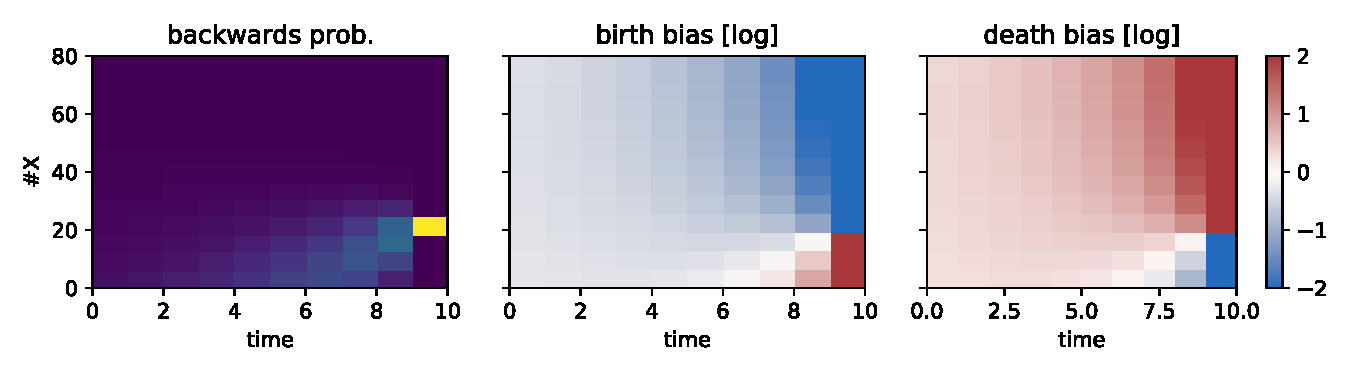
\includegraphics[width=\textwidth]{gfx/biases.pdf}
    \caption[Approximate biasing]{\label{fig:biases}The approximate dynamic biasing (cut to $[e^{-2}, e^{2}]$) illustrated for a birth death process with macro-state size $8$ and target state $[40, 47]$ at $T=10$ for $10$ time points.}
\end{figure}

Using these approximate backwards probabilities we can compute approximate predilections for the aggregated system.

\autoref{fig:biases} clearly illustrates how the biases increase towards the end increasing the push towards the goal state the farther time progresses.
But this is only true in the aggregated system, where we consider macro-states as one unit.
Therefore, we need to transfer the biases back to the original micro-states somehow.
This essentially entails an interpolation between the bias values $\bar{\phi}$.
The simplest way is to use a linear interpolation.
Specifically, we assume the biases to be exactly their approximate value at the center of each macro-state.
Away from these states, we take an average of the adjacent center points weighted by their distance.
\[
    \hat{\phi}_j(x, t) = \sum
\]

Now, that we have a macro-state biasing, we need to transition back to the original system.
The approximation assumes probability mass only to be different between macro-state borders.
Therefore, we cannot naively transition back: Then the biases are zero for all internal states.
The strategy instead is to compute the biases at the macro-state boundaries and then interpolate these values for the interior states using their distance to each border.

\section{Nonhomogeneous Stochastic Simulation}
We are changing the rate bias dynamically over fixed intervals of the time-domain.
Therefore we cannot use the default \ac{SSA}.
With \autoref{alg:ssa_dyn} we present a version of the \acl{SSA} that simulates trajectories of a system with such dynamically changing biases.
The main change is the handling of the time-discrete changes in the loop in \autoref{line:tloop}.
Here it is tested, in which time interval the sampled jump will take place.
Therefore rates are recomputed each time the algorithm jumps forward one time-interval.
\begin{figure}
    \centering
    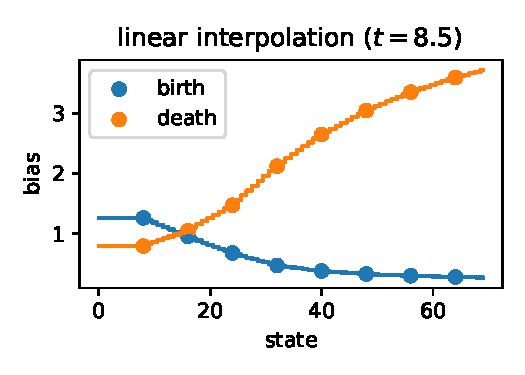
\includegraphics[scale=0.5]{gfx/lin_intp.pdf}
    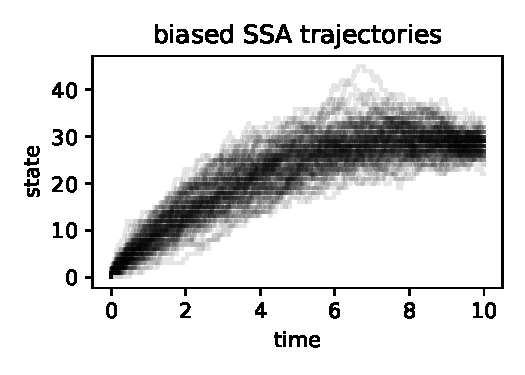
\includegraphics[scale=0.5]{gfx/biased_SSA.pdf}
    \caption[Bias interpolation \& biased \ac{SSA}]{\label{fig:bias_ssa}}
\end{figure}

Let us first consider how exactly the jump time distribution changes.
A time-inhomogeneous exponential has the cdf
\[
    F(t) = 1 - \exp\left(-\int_0^t \lambda(s)\,ds\right)\,.
\]
Accordingly, the pdf
\[
    f(t) = \lambda(t)\exp\left(-\int_0^t \lambda(s)\,ds\right)\,.
\]
Since we compute the biases for fixed intervals, we have a piecewise exponential model.
Assume, we have an increasing sequence of time points $\tau_0=0, \tau_1, \tau_2, \tau_3, \dots$ with corresponding rates $\lambda_i >0$.
The piecewise constant hazard function
\[
    \lambda(t) = \begin{cases}
        \lambda_1, & \text{if } \tau_0 \leq t \leq \tau_1\\
        \lambda_2, & \text{if } \tau_1 < t \leq \tau_2\\
        \lambda_3, & \text{if } \tau_2 < t \leq \tau_3\\
        \quad\vdots
    \end{cases}\,.
\]
We can give the pdf using a case distinction as
\begin{equation}
    f(t) = \begin{cases}
        f_1(t), & \text{if }\tau_0 \leq t \leq \tau_1\\
        f_2(t), & \text{if }\tau_1 < t \leq \tau_2\\
        f_3(t), & \text{if }\tau_2 < t \leq \tau_3\\
        \quad\vdots
    \end{cases}\,,
\end{equation}
where, letting $\Delta_k = \tau_k - \tau_{k-1}$, the piecewise densities
\[
    f_k(t) = \lambda_k \exp \left( -\sum_{i=1}^{k-1}\Delta_i\lambda_i - \lambda_k\left(t - \tau_{k-1}\right)\right)\,.
\]
Similarly, the cdf
\begin{equation}
    F(t) = 1 - \begin{cases}
        S_1(t), & \text{if }\tau_0 \leq t \leq \tau_1\\
        S_2(t), & \text{if }\tau_1 < t \leq \tau_2\\
        S_3(t), & \text{if }\tau_2 < t \leq \tau_3\\
        \quad\vdots
    \end{cases}\,,
\end{equation}
where the component survival functions
\[
    S_k(t) = \exp \left( -\sum_{i=1}^{k-1}\Delta_i\lambda_i - \lambda_k\left(t - \tau_{k-1}\right)\right)\,.
\]
The sampling from this density --~necessary in the stochastic simulation~-- uses an inverse transform.
This transform is most concisely expressed in lines \ref{line:jump_start}--\ref{line:update_t} of the pseudocode in \autoref{alg:ssa_dyn}.
The uniform random sample $X$ is checked against the probability mass of the current time interval.
The mass follows an exponential distribution with the current exit rate $a_0$.
In each iteration we recompute the rate $a_0$ and advance the time until the correct interval is identified.
Finally, in \autoref{line:update_t} the jump time is computed.

Since the jump time is determined after this part, the reaction selection uses the rates of this time-interval.
The probability of a reaction $j$ being selected is proportional to its biased reaction rate $\alpha_{i,j}'$ (\autoref{line:sample_dyn_r}).

The sampling of successive reactions is performed until the predefined termiantion function $\Theta$ is true.
Typically this means reaching some time-horizon $T>0$, i.e.\ $\Theta(s, t)=t>T$.
\begin{algorithm}
\SetKwInOut{Input}{input}
\SetKwInOut{Output}{output}
    \Input{$\pi_0, \theta, \Theta$}
    \Output{sample weighted by the likelihood ratio}
    %$\tau \leftarrow$ empty list\;
    $s\sim\pi_0$; $t\leftarrow 0$; $j\leftarrow 1$; $w\leftarrow 1$\;
    \Loop{\label{line:outer_loop}}{
        %$\tau\leftarrow \text{append}(\tau, (s, t))$\;
        $X\sim U[0,1]$\label{line:jump_start}\;
        $a_0\leftarrow\sum_i\alpha_{i,j}'(s)$\tcc*[r]{exit rate}
        $\delta\leftarrow t_{j+1} - t$\tcc*[r]{rest of time interval}
        $\Delta\leftarrow 0$\tcc*[r]{time offset}
        $\tau \leftarrow t$\tcc*[r]{start of the current component}
        \While{$X>1 - \exp(-a_0 \delta-\Delta)$\tcc*[r]{find interval}\label{line:tloop}}{
            $\Delta\leftarrow \Delta + a_0\delta$\;
            $\tau\leftarrow \tau + \delta$\;
            $j\leftarrow j+1$\;
            $\delta\leftarrow $ time-interval width\;
            $a_0\leftarrow\sum_i\alpha_{i,j}'(s)$\label{line:jump_end}\tcc*[r]{exit rate}
        }
        $\delta \leftarrow - ( \log(1-X) + \Delta )/{a_0}$\;

        \If{$\Theta(s, \tau + \delta)$}{
            \Return $\theta(s, \tau) w$
        }
        $k\leftarrow$ sample $i$ with probability $\alpha_{i,j}'(s)/\sum_i\alpha_{i,j}'(s)$\label{line:sample_dyn_r}\;
        ${\ell}_{1} \leftarrow \alpha_{k,j}'(s) \exp\left(-\Delta - \delta a_0\right)$\;
        ${\ell}_{0} \leftarrow \alpha_k(s) \exp\left(- (\tau + \delta - t) \sum_i\alpha_i(s)\right)$\;
        $w\leftarrow w\; {\ell}_0 / {\ell}_1$\label{line:update_w}\tcc*[r]{update likelihood ratio}
        $t \leftarrow \tau + \delta$\label{line:update_t}\tcc*[r]{update time}
        $s\leftarrow s + v_k$\tcc*[r]{update state}
    }
    \caption{\label{alg:ssa_dyn}A weighted sample of the rare event}
\end{algorithm}

\subsection{Issues}
\begin{itemize}
    \item Works for some models
    \item often: under- or over-acceleration
    \item due to the approximative nature, the speed is often too high or too low
    \item simultions reach the target to early: many samples with very low weight, few with high weight
    \item the estimates are still unbiased but not approximately normally distributed, even for larger biases (make an example, that this is also the case for constant biasing)
    \item bias strength can be adjusted such that only a portion reaches
    \item this improves the somewhat, but may alter the biases too much and the weight distribution (sampled) is still bad
    \item solution: use importance splitting instead
\end{itemize}

\section{Importance Splitting}
\begin{itemize}
    \item newer stuff \parencite{budde2017better}
    \item \ac{RESTART} original paper \parencite{villen1994restart}
    \item fixed effort splitting \parencite{garvels1998comparison}
    \item Legay \cite{jegourel2013importance}
\end{itemize}

\section{Conclusion}
\subsection{Future Work}
\begin{itemize}
    \item \emph{Multiple importance sampling} for different accelerations to avoid problems of under- and overacceleration
\end{itemize}
